\chapter{Uvod}
Adaptivno učenje u e-learning softverima tipično funkcionira tako da mjeri razinu znanja korisnika kroz početni skup pitanja, virtualnu simulaciju i/ili dodijeljene zadatke. Na temelju podataka prikupljenih iz odgovora korisnika, takav softver u stvarnom vremenu procjenjuje razliku između korisničkog znanja i znanja potrebnih za određenu kompetenciju, te odabire lekcije i zadatke za korisnika tako da minimizira količinu edukacijskog sadržaja koji tom korisniku prikazuje.\newline
Konstrukcija algoritma za određivanje puta za adaptivno učenje tipično se radi na dva načina: 1) kreiranjem formalnog modela znanja za određenu domenu, a koji kreiraju eksperti iz te domene ili 2) koristeći algoritamski pristup baziran na teorijama Bayesian Knowledge Tracing i Item Response Theory koji na temelju odgovora polaznika edukacije procjenjuje vjerojatnost da je polaznik usvojio određenu vještinu/koncept (što ponovno zahtijeva unaprijed definirane vještine/koncepte).\newline
U posljednje vrijeme, a s obzirom na dostupnost sve većih količina podataka (big data) ponovno su oživjele i dodatno se razvijaju tehnologije kreiranja grafova znanja (npr. pomoću dubokog učenja), a koji s obzirom na to da su kreirani statistički mogu biti mnogo kompleksniji i uže segmentirani (precizniji) u odnosu na one koje kreiraju eksperti nekog područja. Dodatno, prikupljanje velike količine informacija u različitim domenama omogućuje da kreiranje grafova znanja ne bude ograničeno samo na one tvrtke koje imaju golem broj korisnika kao što su Google ili Facebook. Na temelju inicijalnog istraživanja vjerujemo da se ova metoda može primijeniti i na kreiranje grafova znanja za adaptivno učenje, te time omogućiti s jedne strane znatno veću adaptivnost, a s druge strane veću jednostavnost kreiranja takvih grafova.\newline
Ovo je posebno važno za područja edukacije izvan formalnog obrazovanja, gdje nisu strogo definirane ishodi učenja i testovi kojima se mjeri je li neki ishod učenja dostignut kod pojedinog polaznika. Dva primjera za to su instrukcije, gdje učeniku često nedostaju i predznanja iz drugih područja koje je ranije u školi trebao usvojiti, te korporativne edukacije, koje često obuhvaćaju ljude različitih struka i različitim znanjima iz domene za koju nastoje dobiti certifikat.


\chapter{Cilj i postupak}
Stoga je cilj ovog projekta provjeriti sljedeće:
\begin{itemize}
\item Provjera mogućnosti kreiranja grafa znanja isključivo na temelju točnosti odgovora na zadacima iz jedne domene znanja koje korisnici daju i informacije o redoslijedu zadavanja zadataka pojedinom korisniku
\item Ako je navedeno moguće, potrebno je provjeriti može li se kreirati graf znanja na temelju rješavanja zadataka za istu domenu na temelju parcijalnog broja zadataka (što realnije reprezentira dostupne zadatke za stvarne domene – rijetko su dostupna baš sva znanja iz neke domene da bi se mogla kreirati zadaci koji pokrivaju baš svaku informaciju u toj domeni)
\item Ako je navedeno moguće, potrebno je provjeriti može li se isto napraviti i za neku domenu realnog znanja\newline
\end{itemize}
Ukratko, ovim se projektom provjerava može li se graf znanja potreban za adaptivno učenje kreirati metodama dubokog učenja na temelju ponašanja korisnika na zadacima (probabilistički), a bez potrebe za time da eksperti unaprijed određuju koncepte/vještine u koje se grupiraju zadaci ili čak sam graf znanja.\newline\newline
Za potrebe ove provjere kreirat će se:
\begin{itemize}
	\item umjetni, zatvoreni graf znanja 
	\item zadaci koji pokrivaju sve informacije prisutne u tom zatvorenom grafu znanja\newline
\end{itemize}
Potom će se zadaci dati testerima na rješavanje, tako da se:
\begin{itemize}
	\item varira redoslijed zadataka koje pojedini tester dobiva kako bi pokrio sve kombinacije
	\item bilježi točnost odgovora testera na zadatak
	\item u slučaju netočnog odgovora testeru se prikazuje točna informacija.
\end{itemize}

\chapter{Postojeće ideje i koncepti}
Istraživanjem fraza kao što su Bayesian Knowledge Tracing (BKT), Item Response Theory (IRT), Deep Knowledge Tracing (DKT), Intelligent Tutoring Systems (ITS), Massive Open Online Courses (MOOC), itd. pronađeni su mnogi radovi koji su služili kao sredstvo upoznavanja s tematikom rada i inpiracija za daljnja ostvarenja. 
\newline
\newline
Među prvima pronađena je i proučena platforma adaptivnog učenja Knewton korištena za personalizaciju edukacijskog sadržaja \citep{knewton}. 
\newline
\newline
Izazovnim područjem praćenja znanja (engl. \textit{knowledge tracing}) moguće je strojno modelirati znanje korisnika pomoću njegove interakcije s računalom tijekom procesa učenja \citep{dkt}. Korisnicima je predložen sadržaj učenja ovisno o njihovim potrebama (sadržaj je okarakteriziran kao prelagan, pretežak, moguće ga je potpuno preskočiti ili ostaviti za kasnije). Predviđaju se buduće korisničke performanse prema prošloj aktivnosti. Mnoge metode pri tome uključuju korištenje Markovljevih modela s ograničenom funkcionalnošću. Također, neki modeli koriste logističku regresiju uz PFA (engl. \textit{performance factors analysis}). U novije vrijeme, korištene su povratne neuronske mreže (engl. \textit{recurrent neural networks, RNN}) pa cjelokupni model nosi naziv Deep Knowledge Tracing (DKT). \newline
RNN-ovi su popularni jer imaju petlje i omogućuju opstanak informacije, za razliku od uobičajnih neuronskih mreža. Moguće ih je protumačiti kao mnogostruke kopije iste mreže od kojih svaka predaje poruku idućoj, kao što je vidljivo na slici ~\ref{fig:rnn}.
\pagebreak

\begin{figure}[!htb]
	\centering
	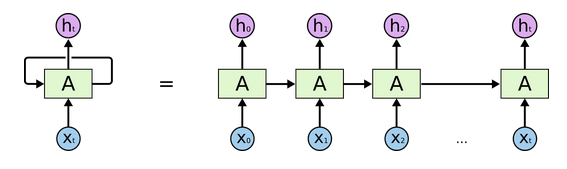
\includegraphics[scale=1]{rnn.png}
	\caption{Intuitivni prikaz povratne neuronske mreže (RNN)}
	\label{fig:rnn}
\end{figure}

Posebice je popularna kompleksnija varijanta RNN-a, LSTM (engl. \textit{long short-term memory}). Interakcije (pitanje-odgovor) potrebno je pretvarati u vektore fiksne duljine (ideja je inpute predstaviti one-hot encodingom parova (oznaka zadatka, točnost)). Mapiranje u izlazne vrijednosti postiže se računom slijeda “skrivenih” stanja (uzastopnim enkodiranjem bitnih informacija proteklih zapažanja kako bi odgovarale budućim predikcijama). Izlazna vrijednost je vektor vjerojatnosti točnog rješavanja svakog od zadataka u modelu. 
Sposobnost predviđanja korisničkih performansi ispitana je na simuliranom skupu podataka. Umjetno su generirani korisnici koji rješavaju određen broj zadataka iz fiksnog skupa koncepata. Svaki korisnik ima latentnu “vještinu” za svaki koncept, a svaki zadatak ima koncept i težinu. Vjerojatnosti da korisnik točno riješi zadatak određene težine ako ima određenu vještinu modelirane su pomoću IRT-a. Također, otkriven je javno dostupan benchmark skup podataka, 2009-10 Assistments Data.
\newline
\newline
Ponađen je i proučen i sustav KnowEdu, kojem je cilj konstruirati grafove znanja za edukacijske potrebe i identificirati odnose između različitih koncepata \citep{knowedu}.\newline
Na početku se pokušavaju ustanoviti svi koncepti koji se nalaze u dostupnim nastavnim materijalima i tečajevima korištenjem strojnog učenja. Zatim se koriste CRF (engl. \textit{conditional random field}) model, povratna neuronska mreža i varijanta LSTM mreže, GRU (engl. \textit{gated recurrent units}) kako bi se dobio graf preduvjeta. Skup podataka prikupljen je iz više testova pri čemu je svaki ispitanik riješio svaki test. Jedan test sastoji se od više pitanja koja ispituju znanje istog koncepta i pomoću njega se izračuna odgovarajuća ocjena znanja tog koncepta za svakog ispitanika. Ocjene predstavljaju vještine ispitanika u tom području i one su ulaz modela. Svaki model kao izlaz daje, za svaku kombinaciju koncepata, vjerojatnost da je koncept A preduvjet za znanje koncepta B.